\documentclass{beamer}
\mode<presentation>
{
  \usetheme{Warsaw}
  \definecolor{mcgarnet}{rgb}{0.38, 0, 0.08}
  \definecolor{mcgray}{rgb}{0.6, 0.6, 0.6}
  \setbeamercolor{structure}{fg=mcgarnet,bg=mcgray}
  %\setbeamercovered{transparent}
}


\usepackage[english]{babel}
\usepackage[latin1]{inputenc}
\usepackage{times}
\usepackage[T1]{fontenc}
\usepackage{tikz}
\usepackage{graphicx}
\usepackage{amsmath}
\usepackage{adjustbox}
\usepackage{fancyvrb}

\newcommand{\imagesource}[1]{{\centering\hfill\break\hbox{\scriptsize Image Source:\thinspace{\small\itshape #1}}\par}}

\title{02 - Math Preliminaries}


\author{Dr. Robert Lowe\\}

\institute[Maryville College] % (optional, but mostly needed)
{
  Division of Mathematics and Computer Science\\
  Maryville College
}

\date[]{}
\subject{}

\pgfdeclareimage[height=0.5cm]{university-logo}{images/Maryville-College}
\logo{\pgfuseimage{university-logo}}



\AtBeginSection[]
{
  \begin{frame}<beamer>{Outline}
    \tableofcontents[currentsection]
  \end{frame}
}


\begin{document}

\begin{frame}
  \titlepage
\end{frame}

\begin{frame}{Outline}
  \tableofcontents
\end{frame}


% Structuring a talk is a difficult task and the following structure
% may not be suitable. Here are some rules that apply for this
% solution: 

% - Exactly two or three sections (other than the summary).
% - At *most* three subsections per section.
% - Talk about 30s to 2min per frame. So there should be between about
%   15 and 30 frames, all told.

% - A conference audience is likely to know very little of what you
%   are going to talk about. So *simplify*!
% - In a 20min talk, getting the main ideas across is hard
%   enough. Leave out details, even if it means being less precise than
%   you think necessary.
% - If you omit details that are vital to the proof/implementation,
%   just say so once. Everybody will be happy with that.

\section{Relations}
\begin{frame}{Relation}
\begin{itemize}
    \item<2-> A \textbf{relation}, $R$ between two sets, $A$ and $B$ is:
    \[
        R \subset A \times B
    \]
    \item<3-> For example, consider the $<$ relation:
    \begin{align*}
       \uncover<4->{\textrm{\textbf{Let} } S=&T=\{1,2,3\}\\}
       \uncover<5->{S \times T =& \{(1,1), (1,2), (1,3), \\
                               & (2,1), (2,2), (2,3), \\
                               & (3,1), (3,2), (3,3)\}} \\
       \uncover<6->{U=& \{(1,2), (1,3), (2,3)\}}
    \end{align*}
    \uncover<7->{Thus $U$ is the sought after $<$ relation!}
    \item<8-> We often write relations this: $aUb$ where $aUb$ is true if
        and only if $(a,b) \in U$
\end{itemize}
\end{frame}

\begin{frame}{Digraphs}

A {\bf digraph} is a graphical representation of a relation.
\begin{center}
    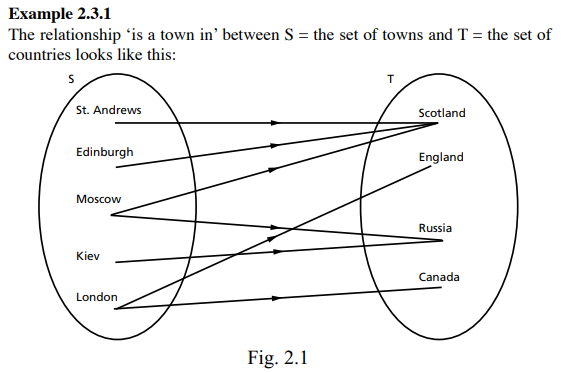
\includegraphics[height=0.70\textheight]{images/digraph}
    {\tiny From Davie and Morrison page 26}
\end{center}
\end{frame}

\begin{frame}{Properties of Relations}
\begin{itemize}[<+->]
    \item $A$ \textbf{includes} $B$ if, $\forall s \in S$ and $t \in T$,
        $sBt \implies sAt$
    \item $A$ is the \textbf{transpose} of $B$ if, $\forall s \in S$ and 
        $t\in T$, $sAt \iff tBs$
    \item $A$ is \textbf{reflexive} if $S=T$ and $\forall s \in S$,
        $sAs$ is true.
    \item $A$ is \textbf{transitive} if $S=T$ and 
        $\forall r,s,t \in R,S,T$, $rAs \textrm{ and }sAt \implies rAt$
\end{itemize}
\begin{block}{Exercise}<+->
    For each of the above properties, define a relation that exhibits
    this property.
\end{block}
\end{frame}

\begin{frame}{Algebra of Relations}
    \begin{itemize}[<+->]
        \item Let $A$ be a relation between $R$ and $S$. 
            ($A\subset R \times S$)
        \item Let $B$ be a relation between $S$ and $T$.
            ($B\subset S \times T$)
        \item The \textbf{product} $AB \subset R \times T$ is defined as: 
            $rABt \iff \exists s \in S : rAs \textrm{ and } sBt$
        \item This product is associative but not commutative.
        \item The equality relation, $I$, is the identity
        \[
            I_sA = A = A I_t
        \]
        \item We define \textbf{powers} of $A$ as:
        \begin{itemize}
            \item $A^0 = I$
            \item $A^{n+1} = A^nA$ for $n > 0$
        \end{itemize}

    \end{itemize}
\end{frame}


\section{Closures of Relations}
\begin{frame}{Transitive Closure}
    \begin{itemize}[<+->]
        \item let $A \subset S \times S$
        \item The transitive closure of $A$ is:
        \[
            A^+ = \displaystyle\sum_{i=1}^{\infty} A^i
        \]
        \item Finite closures exist when $A^+$ converges.

    \end{itemize}
\end{frame}

\begin{frame}{Reflexive Transitive Closure}

    Adding $I=A^0$ to $A^+$ yields the reflexive transitive closure of
    $A$.
        \[
            A^* = \displaystyle\sum_{i=0}^{\infty} A^i
        \]
\end{frame}

\begin{frame}{Example: Direct Divisor Relation}
    \begin{itemize}[<+->]
        \item Let $S=T=$ the set of divisors of 12.
        \item The direct divisor relation is
            \newline$\{(1,2),(1,3),(2,4),(2,6),(3,6),(4,12),(6,12)\}$
        \item This relation's digraph is:
            \newline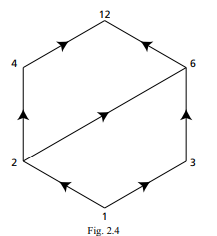
\includegraphics[height=4cm]{images/divisor-graph}
            \newline{\tiny (Davie and Morrison page 30)}
    \end{itemize}
\end{frame}

\begin{frame}{Example: Binary Matrix of Direct Divisor Relation}
    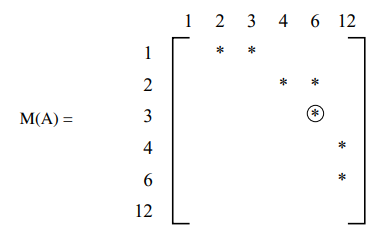
\includegraphics[height=4cm]{images/divisor-binmatrix}
    \newline{\tiny (Davie and Morrison page 30)}
\end{frame}

\begin{frame}{Adding Binary Matrix Representations of Relations}
    \begin{itemize}[<+->]
        \item $M(A+B) = M(A) \vee M(B)$
        \item Let's compute $M(A^2)$
        \item Next, compute $M(A+A^2)$
        \item Let's compute $A + A^2 + \ldots$ until it ``settles
        down''
        \item This gives us $A^+$, to get $A^*$ we just make all
        diagonal elements true.
    \end{itemize}
\end{frame}

\begin{frame}[fragile]{Computing transitive closure in S-Algol}
\begin{adjustbox}{max width=0.9\textwidth}
\begin{BVerbatim}
!Read or calculate bool matrix A(nxn)
for i=1 to n do     !Each time round, add a new node
                    !(number i) to the transitive closure graph
  for j=1 to n do   !Find all arrows leading into node i
  if A(j,i) do      !If there is an arrow from node j to node i,
                    !find all those out of node i
    for k=1 to n do !make a direct path arrow between nodes j
        A(j,k):=A(j,k) or A(i,k)
                    !Now A contains the transitive closure matrix
\end{BVerbatim}
\end{adjustbox}

{\tiny From Davie and Morrison page 33}
\end{frame}

\end{document}


